\begin{frame}{Introduction to the data assimilation}
 Data assimilation is widely used in:
 \begin{enumerate}[\textbullet]
		\item weather forecastinf
		\item ocean simulation
 \end{enumerate}	 
   	The main idea of the data assimilation is to combine:
 \begin{enumerate}[\textbullet]
		\item a model
		\item some observations
 \end{enumerate}	 
 The best estimation:
 $$x^a=Lx^b+Ky^0$$
 with $x^a$ the analyzed state, $x^b$ the state of the model and $y^0$ the observations.
\end{frame}
\subsection{Theory}
\begin{frame}[allowframebreaks]{Kalman filter}
    The Kalman filter method consists in looking for $x^a$ an analysis, this analysis will be a linear combination of what our model and our observations.
    $$x^a=x^b+K(y-x^b)$$
    with K the gain matrix.
    \newline Let’s consider that we are in 1D, and true state $x^t$ exists:
    $$x^a-x^t=x^b-x^t+K(y-x^t-x^b+x^t)$$
	Errors:
    $$\begin{aligned}
        &\epsilon^a=x^a-x^t, \\
        &\epsilon^b=x^b-x^t, \\
        &\epsilon^y=y-x^t, \\
    \end{aligned}$$
    \newpage
    We can also write:
    $$<\epsilon^a>=<\epsilon^b>+K(<\epsilon^y>-<\epsilon^b>)$$
    Analysis error variance as low as possible.
    \newline Minimize $<(\epsilon^a)^2>$ with respect to $K$ :
    $$<(\epsilon^a)^2>=<(\epsilon^b)^2>+K^2<(\epsilon^y-\epsilon^b)^2>+2K<\epsilon^b(\epsilon^y-\epsilon^b)^2>$$
    The errors in the background and observation are uncorrelated.
    $$K=\frac{<(\epsilon^b)^2>}{<(\epsilon^b)^2>+<(\epsilon^y)^2>} \Rightarrow K=\frac{(\sigma^b)^2}{(\sigma^b)^2+(\sigma^y)^2} $$
    $(\sigma^y)^2$ the observation error variance, \newline $(\sigma^b)^2$ the background or model error variance.

	\newpage
    Now that we have explained the method for finding $x^a$ let's try to generalize our formula in a multi-dimensional case.

    $$\left\{\begin{aligned}
  &x^a=(I-KH)x^b+Ky^0=x^b+K(y^0-H(x^b)) \\
        &K=BH^T(HBH^T+R)^{-1} \\
 \end{aligned}\right.$$
    With $K$ the gain or weight matrix.
    This formulation is called the Best Linear Unbiased Estimator (BLUE).

	\newpage

    \pgfimage[height=5.5cm,width=11cm]{images/schema_kalman_filter.png}
\end{frame}
\begin{frame}{Minimizing a cost function}
    Solves the analysis problem through an optimisation (minimisation of a cost-function)
    Variational approach of BLUE consists in finding $x^a=\arg\max_{x}J$:
    $$\begin{aligned}
        J(x)&=\frac{1}{2}(x^b-x)^TB^{-1}(x^b-x)+\frac{1}{2}(y-H(x))^TR^{-1}(y-H(x)) \\
        &=\frac{1}{2}\|x-x^b\|_B^2+\frac{1}{2}\|H(x)-y^0\|_R^2
    \end{aligned}$$
	\begin{minipage}{\linewidth}
		\centering
		\pgfimage[width=0.6\linewidth]{images/schema_3D_Var.png}
	\end{minipage}
\end{frame}
\begin{frame}{Ensemble Filter Kalman}
    The ENKF method consists in using the Kalman filter method in high dimension.
    \newline We apply the Kalman filter on several state samples $x_1,x_2,..,x_{m}$.
    $$x_i^a=x_i^f+K[y-h(x_i^f)]$$
    with $h(x_i^f)$ the observation operator.
    We can also define the Kalman gains: 
    $$K=P^f H^T(HP^f H^T+R)^{-1}$$
    For exemple we can estimate the
    forecast error covariance matrix as:
    $$P^f=\frac{1}{m-1}\sum_{i=1}^{m}(x_i^f-\bar{x}^f)(x_i^f-\bar{x}^f)^T~~\text{with}~~\bar{x}^f=\frac{1}{m}\sum_{i=1}^{m}x_i^f $$ .
\end{frame}
\subsection{Results}
\begin{frame}[allowframebreaks]{Harmonic oscillator}
    $$\qquad \frac{\partial x}{\partial t}=v \quad \Rightarrow \quad \frac{\partial^2 x}{\partial t^2}=\frac{\partial v}{\partial t}$$
    \begin{enumerate}[\textbullet]
		\item We choose for the initial point $(2,0)$
		\item For the period let's take Pe=$\frac{2\pi}{w}$ with $w$ the first components of our initial point
		\item For the discretisation,  dt=$\frac{\text{Pe}}{20}$ 
		\item We try to find the solution in the interval $[0,T]$ with T=$3\text{Pe}$
   	\end{enumerate}

	\newpage

	\; \\

	\begin{figure}[H]
		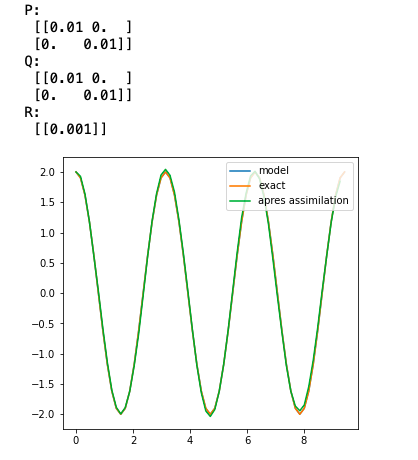
\includegraphics[width=0.32\linewidth]{"images/oscillator1.png"}
		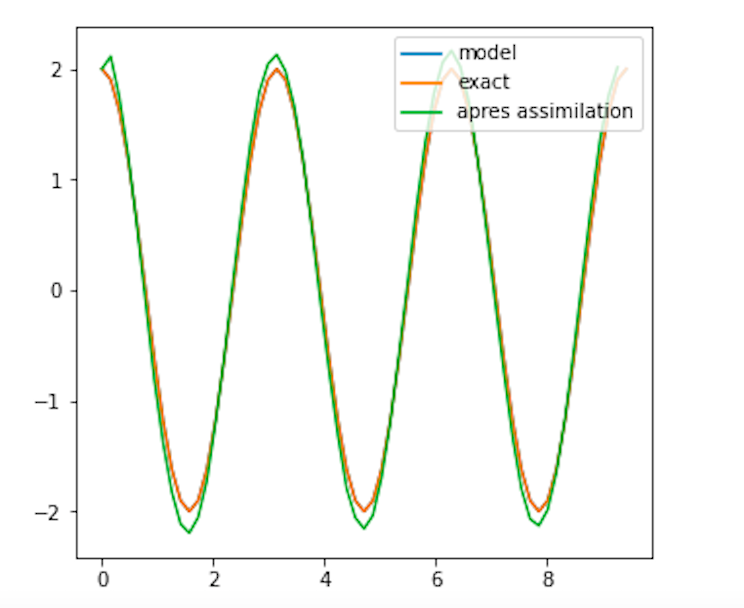
\includegraphics[width=0.32\linewidth]{"images/oscillator2.png"}
		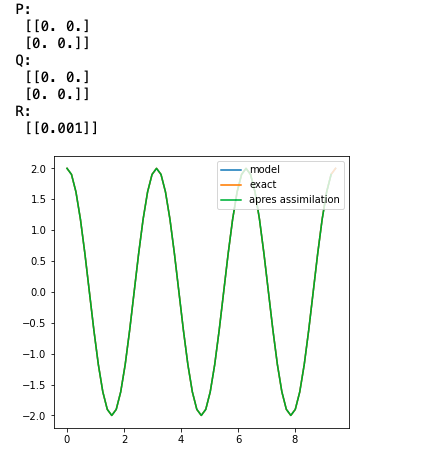
\includegraphics[width=0.32\linewidth]{"images/oscillator3.png"}
	\end{figure}
    
    
\end{frame}
\begin{frame}[allowframebreaks]{Lorenz System}
    $(\sigma, r, b)=(12.,6.,12.)$, $\quad X_0=(-10.,-10.,25.)$, $\quad [t_0,T]=[0,1]$,
	$$P=\begin{pmatrix}
    0.1 & 0. & 0. \\
    0. & 0.1 & 0. \\
    0. & 0. & 0.1 \\
    \end{pmatrix} ,
    Q=\begin{pmatrix}
    0.1 & 0. & 0. \\
    0. & 0.1 & 0. \\
    0. & 0. & 0.1 \\
    \end{pmatrix},
    R=\begin{pmatrix}
    0.01 & 0. & 0. \\
    0. & 0.01 & 0. \\
    0. & 0. & 0.01 \\
    \end{pmatrix}.$$ 
	\pgfimage[width=1.002\linewidth]{images/lorenz_1.png} 
	
	\newpage
	
    \begin{enumerate}[\textbullet]
		\item Model $(\sigma, r, b)=(10.,6.,10.)$, Observation $(\sigma, r, b)=(12.,6.,12.)$,
	    \item $X_0=(-10.,-10.,25.)$, $\quad \Delta t=0.1s$ $\quad [t_0,T]=[0,4]$,
	    \end{enumerate}
    	$$P=\begin{pmatrix}
        0.1 & 0. & 0. \\
         0. & 0.1 & 0. \\
        0. & 0. & 0.1 \\
        \end{pmatrix} ,
        Q=\begin{pmatrix}
         0.01 & 0. & 0. \\
        0. & 0.01 & 0. \\
        0. & 0. & 0.01 \\
        \end{pmatrix},
        R=\begin{pmatrix}
        0.1 & 0. & 0. \\
        0. & 0.1 & 0. \\
        0. & 0. & 0.1 \\
        \end{pmatrix}.$$

	\begin{figure}
		\centering
		\pgfimage[width=0.89\linewidth]{images/lorenz_2.png}
	\end{figure}

	\newpage
 
	\begin{enumerate}[\textbullet]
	     	\item Model $(\sigma, r, b)=(10.,6.,10.)$,Observation $(\sigma, r, b)=(12.,6.,12.)$,
	        \item $X_0=(-10.,-10.,25.)$, $\quad \Delta t=0.1s$ $\quad [t_0,T]=[0,4]$,
	\end{enumerate}
    $$P=\begin{pmatrix}
    0.1 & 0. & 0. \\
    0. & 0.1 & 0. \\
    0. & 0. & 0.1 \\
    \end{pmatrix} ,
    Q=\begin{pmatrix}
    0.1 & 0. & 0. \\
    0. & 0.1 & 0. \\
    0. & 0. & 0.1 \\
    \end{pmatrix},
    R=\begin{pmatrix}
    0.01 & 0. & 0. \\
    0. & 0.01 & 0. \\
    0. & 0. & 0.01 \\
    \end{pmatrix}.$$ 

	\begin{figure}
		\centering
    	\pgfimage[width=0.89\linewidth]{images/lorenz3_b.png} 
    \end{figure}
\end{frame}
	